
This chapter describes the controller design used for setpoint regulation. To this end, a Jacobian controller is implemented with some additional features. The controller as presented here is a variation as the one presented in \cite{MOOSAVIAN20071226}. Furthermore, the control architecture in which the Jacobian controller operates is elucidated. The experimental set-up allows to regulate pressure levels as well. Therefore the high-level Jacobian controller is ran at low bandwidth and supported 







To control the dynamic system a Jacobian controller is proposed. The method implemented uses the Jacobian transposed as presented in . This work shows that a computed torque controller can be approximated by a more straightforward control law involving the Jacobian transpose. This approximation holds if high enough control gains are used. This Jacobian transposed control law is given by,

\begin{equation}
    \tau = J^\top (K_p e + K_d \dot{e}) \hspace{10pt} \text{with}  \hspace{10pt} \dot{x} = J\dot{q}
    \label{eq:tau}
\end{equation}

where $\tau$ is the input force, $J$ the Jacobian matrix as expressed in (\ref{eq2:J}). Furthermore, $K_p \in \mathbb{R}^{2\times 2}$ and $K_d \in \mathbb{R}^{2\times 2}$ are diagonal gain matrices that correct for the error and the error derivative expressed in task space variables, respectively. 

It is our goal to control the end-effector position of the soft robotic manipulator. To this end, Jacobian at the end-effector needs to be known. An expression for the end-effector Jacobian is given in \cite{Boyer2019} as,

\begin{equation}
    J(\sigma) = \text{Ad}^{-1}_{g(\sigma)} \int_0^\sigma \text{Ad}_g(s) B_a \Phi(s)d\sigma
\end{equation}


where $\text{Ad}_g$ and  $\text{Ad}^{-1}_g$ are the adjoint and inverse adjoint mapping for position vector $g$ at instance $s$, respectively. Although the length of the actuator varies, we assume $\sigma$ equal to undeformed actuator length $L_0$. Matrix $\text{B}_a$ is a selection matrix of free strains and curvatures. Shape function matrix $\Phi(s)$ evaluates the shape function at instance $s$. In the dynamic simulations this Jacobian is updated at every time instant given the robot configuration. This allows us to include model information to our control law.  In an effort to improve tracking performance. For the real life control system we are aiming to recreate the state with the means of sensors. In this way the Jacobian can be calculated in real-time while carrying out a reference trajectory.













\section{Pump Dynamics}


\begin{theorem}
It is assumed that both air pumps have the equal pump characteristics
\end{theorem}


Besides soft robot actuator properties also the actuator properties need to be involved. To this end pump dynamics need to be determined. In the proposed control architecture, the high level Jacobian controller is accompanied by a lower level pressure controller. The reference pressure is determined by the Jacobian controller by some force to pressure mapping. To this end, the pump dynamics need to be determined. Initially, we solely determine the pump dynamics. Using this dynamics will result to poor performance once connected to the soft actuator. To suppress noise levels and provide capture the actual system dynamics the set-up is slightly adapted.

To determine the pump dynamics the pump is connected directly to the pressure sensor using a short flexible silicone hose. The pump is powered by an electric 12V DC motor, and uses membranes to create pressure. The pump characteristics are obtained by observing the systems response for various volt step inputs between 1 and 6 Volt. Although the pumps are able to operate at 12 Volt, only a maximum step input of 6V is possible for this set-up. The pressure sensor measures absolute pressures between 0 and 25 PSI, which is equivalent to a maximum of 172 kPa. Depending on weather conditions, the maximum theoretically measurable pressure is around 72 kPa. However, experiments have shown results up to 80 kPa are possible. The volt input is regulated via pulse width modulation (PWM). Since the Raspberry PI is equipped with a 12bit ADC (analog-digital converter), it is possible calculate the PWM input as, $\textit{PWM} = \frac{2^{12} V}{V_{max}} $, where $V_{max}$ is equal to 12 volt.  The resulting step responses are shown in Figure (\ref{fig1:pump_dynamcis}).

\begin{figure}[H]
    \centering
    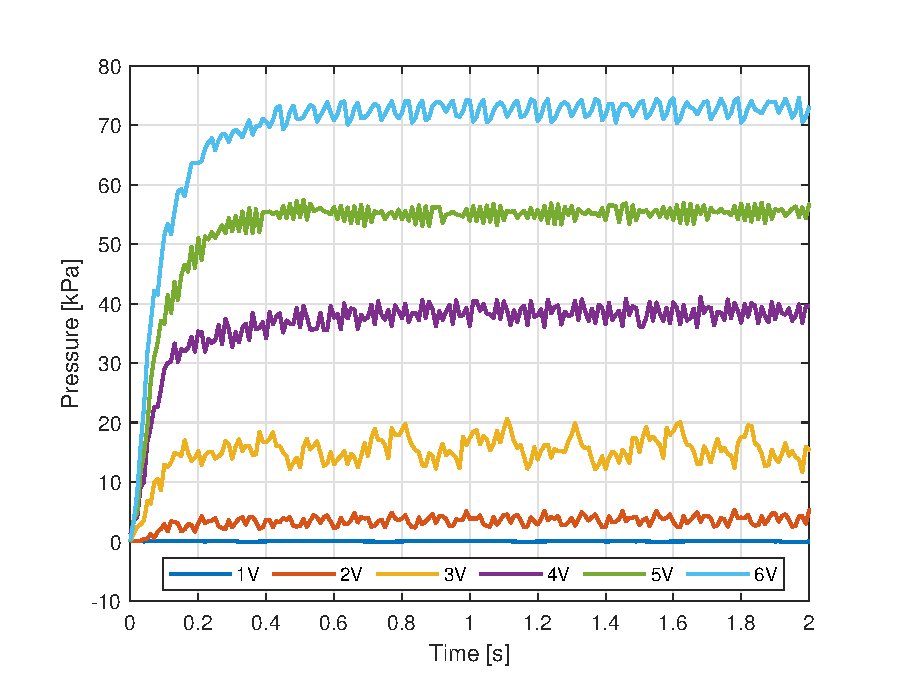
\includegraphics[width = 0.6\textwidth]{Figures/Chapter3/stepresponsdirect16V.eps}
    \caption{Step response for volt step input between 1V and 6V.}
    \label{fig1:pump_dynamcis}
\end{figure}

From Figure (\ref{fig1:pump_dynamcis}) multiple observations can be made. The step response indicates first order system behaviour as the pressure increase is proportional to the actual pressure. However, the steady-state pressure is not proportional to the input volt. The reason for this behaviour is friction. For 1 and 2 volt input static friction dominates, resulting in no to very small pressure increase.
At 3 volt the transition between dry and kinetic friction is observed. The first order system characteristic becomes more visible, although the pressure response is chattering. Furthermore, we see a rise time of comparable order for step inputs of 4V and above. After around 0.5 seconds the steady-state pressure is reached. For all step inputs oscillations are observed around the steady-state pressure. This phenomena is caused by the fact that there is almost no passive leakage from the small control volume. When the pump valves open and air is pressed into the system the air waves are created. For the step input of 5 volt the valve dynamics can be clearly seen, as the dense red spikes.

An improved pump model can be made by altering the set-up. To this end, the actuator and an air vessel are connected to the system. Previous research showed that adding an air vessel will reduce oscillatory behaviour, at the cost of bandwidth \cite{proper}. The air vessel will increase the control volume of the entire system. When the valves open and additional air is pressed in the system, the relative pressure change is smaller. Additionally, when the actuator expands the relative volume increase will also be smaller. This will cause the system to respond slower to a step input. Furthermore, the maximum achievable pressure is lower. The addition of air vessel and actuator will increase the passive leakage of the system.

For the adapted system the step response is determined for volt steps between 2 and 12 volt. The results are shown in Figure \ref{fig3:pump_dynamics_adapted}.

\begin{figure}[H]
    \centering
    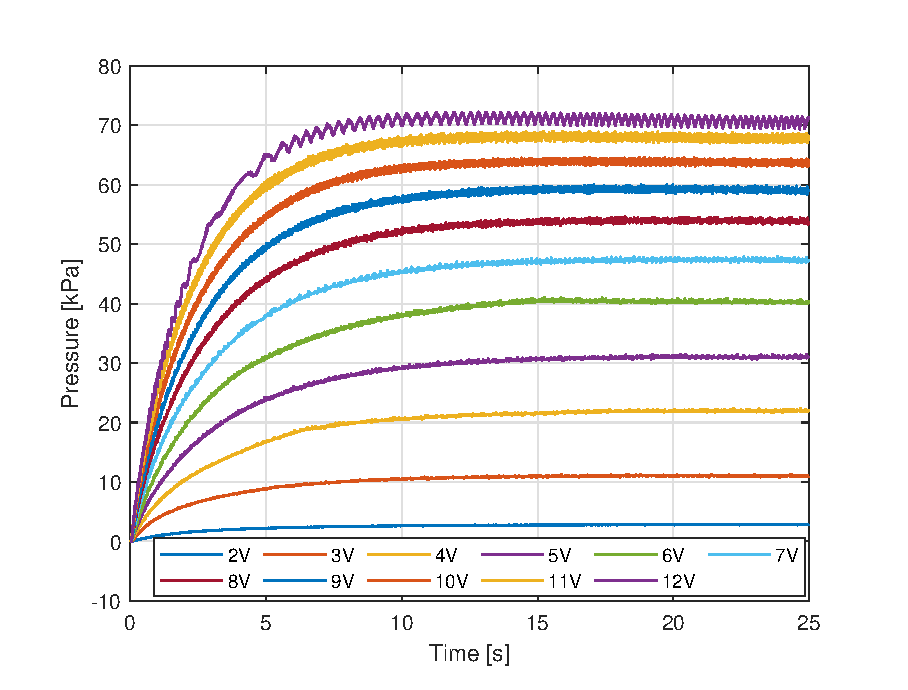
\includegraphics[width = 0.6\textwidth]{Figures/Chapter3/step212V.eps}
    \caption{Step response for volt step input between 2V and 12V for the system including air vessel and actuator.}
    \label{fig3:pump_dynamics_adapted}
\end{figure}


Based on the step responses of Figure (\ref{fig3:pump_dynamics_adapted}) we try to capture the pump dynamics in a model. The time response of a first order linear system responding to a step input is given by, 

\begin{equation}
    p(t,V) = K(1-e^{-t/\tau})V,
    \label{eq3:firstordermodel}
\end{equation}

where $p$ is the pressure at time $t$ in kPa. And constant DC gain $K$ [kPa/V] determines the maximum pressure, time constant $\tau$ [1/s] determines the growth rate of the exponential function. Furthermore, $V$ is the input volt. 

An attempt to fit the linear first order model of (\ref{eq3:firstordermodel}) did not result in an accurate description of the pump dynamics for all step inputs. Therefore an alternative description of the pump dynamics is proposed. In this description constant $K$ is replaced by a nonlinear function $K(V)$. Additionally, a linear function $\tau(V)$ is proposed. 

Based on (\ref{eq3:firstordermodel}) an indication of the gradient between constant $K$ and $V$ can be estimated. The steady-state pressure for each step is estimated by taken the mean over the last 10 seconds of the step response. This pressure is then divided by the corresponding volt input. A similar approach is done for determining time constant $\tau$. For a first order system it can be proven that this time constant is equal to time at which 63\% of the steady state value is reached. The corresponding relations for $K(V)$ and $\tau(V)$ are shown in Figure \ref{fig3:Kest} and Figure \ref{fig3:tauest}, respectively.

\begin{figure}[H]
\begin{minipage}[b]{0.48\linewidth}
\centering
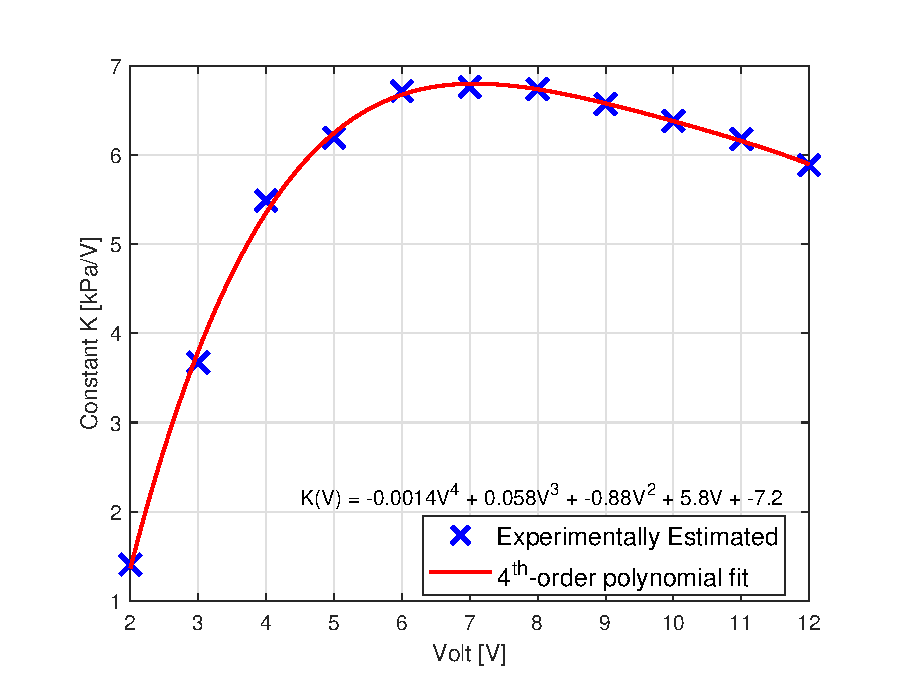
\includegraphics[width=\textwidth]{Figures/Chapter3/Kest.eps}
\caption{Experimental estimate of `constant' $K$ and fourth order fit.}
\label{fig3:Kest}
\end{minipage}
\begin{minipage}[b]{0.48\linewidth}
\centering
\includegraphics[width=\textwidth]{Figures/Chapter3/tauest.eps}
\caption{Experimental estimate of time `constant' $\tau$ and linear fit.}
\label{fig3:tauest}
\end{minipage}
\end{figure}

Figure (\ref{fig3:Kest}) shows a fourth-order polynomial fit to DC-gain $K$. For this fit all data samples were used. Figure (\ref{fig3:tauest}) shows that the estimated time constants for 2 and 3 volt do not follow linear trend line from 4 volt and above. Therefore, in determining the time `constant' $\tau$, only data point from 4 volt onward are used. A possible explanation for these outliers is the friction acting at these voltage inputs, and are therefore not reliable. Furthermore, from a physical point of view, relating time constant $\tau$ to input $V$ is doubtful. Instead, one would prefer defining $\tau$ based on system parameters. However, from a modelling point of view, this method allows to capture the actual model dynamics fairly accurate.

The obtained measurement fits for $K$ and $\tau$ can be substituted in (\ref{eq3:firstordermodel}) resulting in an expression as,

\begin{equation}
    p(t,V) = K(V)(1-e^{-t/\tau(V)})V.
    \label{eq3:firstodernonlinearmodel}
    \end{equation}

The derived first order model of (\ref{eq3:firstodernonlinearmodel}) can be plotted against the experimental results of Figure (\ref{fig3:pump_dynamics_adapted}), this is shown in Figure (\ref{fig3:expvsfitpres}).

\begin{figure}[H]
    \centering
    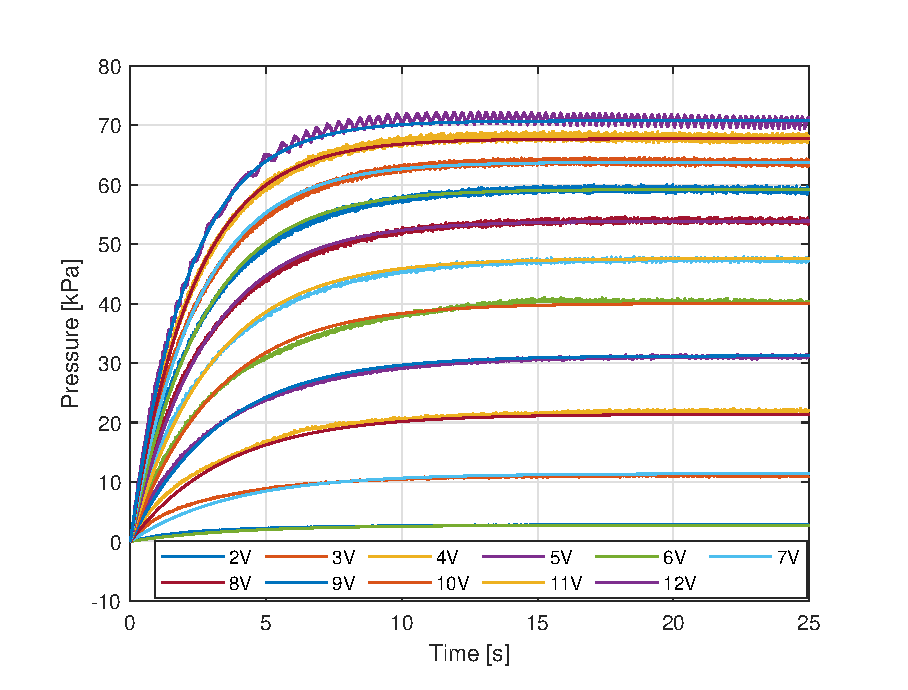
\includegraphics[width = 0.8\textwidth]{Figures/Chapter3/expfit.eps}
    \caption{Experimental results and the derived nonlinear pressure model.}
    \label{fig3:expvsfitpres}
\end{figure}

Above figure shows that the derived model captures the behaviour of the system with actuator and air vessel accurately. The steady-state pressure is close to the experimental value for all volt step inputs. As expected, the rise time for the 1 and 2 volt step inputs are not captured that well by this model.
